\chapter{Temperature distribution with BEM}

\modinfo{Directory}{PoissonBEM}
\modinfo{Solvers}{\Idx{PoissonBEMSolver}}
\modinfo{Tools}{\Idx{ElmerGrid}, editor}
\modinfo{Dimensions}{2D}

\subsection*{Case definition}
This tutorial uses boundary element method (\Idx{BEM}) to solve Poisson equation.
Even though Elmer is primarily a finite element software the are limited
support also for BEM computation. One should however note that Elmer does not
include any multilevel strategies essential for a good performance.
For more details about BEM check the Elmer Models Manual.
The simulation setting is described in Figure~\ref{f:simulationSetting}. 
A heater with constant heat flux is placed inside a box and the walls of the box are in 
fixed temperature.
We are interested in the temperature distribution in the medium around the heater ($\Omega$)
and on the surface of the heater ($\Gamma_1$). We also want to know the heat flux through the
walls of the box ($\Gamma_2$).
\begin{figure}[!htb]
\begin{center}
\setlength{\unitlength}{0.17cm}
\begin{picture}(30,30)
% box walls  *****************
\put(0,0){\line(1,0){30}}
\put(0,30){\line(1,0){30}}
\put(0,0){\line(0,1){30}}
\put(30,0){\line(0,1){30}}
% heater walls ***************
\put(10,10){\line(1,0){10}}
\put(10,20){\line(1,0){10}}
\put(10,10){\line(0,1){10}}
\put(20,10){\line(0,1){10}}
% some text ******************
\put(11,25){$\Omega$, medium}
\put(12.5,14.5){heater}
\put(10,7.5){$\Gamma_1$, $-\frac{\partial T}{\partial n} = 1$}
\put(11,1){$\Gamma_2$, $T=0$}
\end{picture}
\end{center}
\caption{Simulation setting}
\label{f:simulationSetting}
\end{figure}

\subsection*{Solution Procedure}
First we create a mesh with ElmerGrid. The mesh is defined in
{\tt heater.grd} and it is created with command
\ttbegin
ElmerGrid 1 2 heater
\ttend
The solver input file {\tt PoissonBEM.sif} starts with 
the definition of the mesh directory. 
\ttbegin
Header
  Mesh DB "." "heater"
End
\ttend
The simulation uses 2D Cartesian geometry, searches a steady state and since
there is no coupled solvers only one iteration is needed.
Numerical results for restart are written to file {\tt BEM\_Temperature.result}
and file for Paraview visualization is {\tt BEM\_Temperature.vtu}.
\ttbegin
Simulation
  Coordinate System =  Cartesian 2D
  Coordinate Mapping(3) = 1 2 3

  Simulation Type = Steady
  Steady State Max Iterations = 1

  Output Intervals = 1
  Post File = "BEM_Temperature.vtu"
  Output File = "BEM_Temperature.result"
End
\ttend
There is just one body, the medium around the heater, and it uses equation 1.
\ttbegin
Body 1
  Name = "medium"
  Equation = 1
End
\ttend
In equation block we say that we use the solver named {\tt PoissonBEM}.
\ttbegin
Equation 1
  PoissonBEM = Logical True
End
\ttend
In solver block the {\tt Equation} keyword must match the one in equation block.
We also need to define the procedure, name the variable ({\tt Temperature}) and tell 
the degrees of freedom of the variable. Keyword {\tt Optimize Bandwidth} must be set to false
with BEM solver. Since we were interested in the flux, we must now export it to the
results. The lines beginning {\tt Exported} must be exactly as below. Keywords beginning
{\tt Linear System} can be used except that the preconditioning cannot be ILU.
\ttbegin
Solver 1
  Equation = PoissonBEM
  Procedure = "PoissonBEM" "PoissonBEMSolver"
  Variable = Temperature
  Variable DOFs = 1

  Optimize Bandwidth = False

  Exported Variable 1 = String Flux
  Exported Variable 1 DOFs = 1

  Linear System Solver = Iterative
  Linear System Iterative Method = BiCGStab
  Linear System Preconditioning = Jacobi
  Linear System Max Iterations = 100
  Linear System Convergence Tolerance = 1.0e-8

  Steady State Convergence Tolerance = 1.0e-6
End
\ttend
Finally we give the boundary conditions for the heater surface and for the walls of the 
box. The keyword {\tt Body Id} tells the reference body of this boundary. Here it is 1. 
The keyword {\tt Normal Target Body} tells the direction of the outer normal. Value -1 
means the side where there are no volume elements. We didn't mesh the inside of 
the heater and so we can use value -1 in both cases. The heat flux from heater to
medium is 1 and the walls of the box are set to zero temperature. The keyword
{\tt Temperature} matches the name of the variable in solver block.
\ttbegin
Boundary Condition 1
  Name = "heater_surface"
  Target Boundaries = 1

  Body Id = 1
  Normal Target Body = Integer -1
  Flux = Real 1
End

Boundary Condition 2
  Name = "box_walls"
  Target Boundaries = 2

  Body Id = 1
  Normal Target Body = Integer -1
  Temperature = 0
End
\ttend
\subsection*{Results}
Problem is solved with command {\tt Solver}. The results are here viewed with
{\tt ElmerPost}. In Figure~\ref{f:temperature} is the temperature distribution.
\begin{figure}[!hb]
\begin{center}
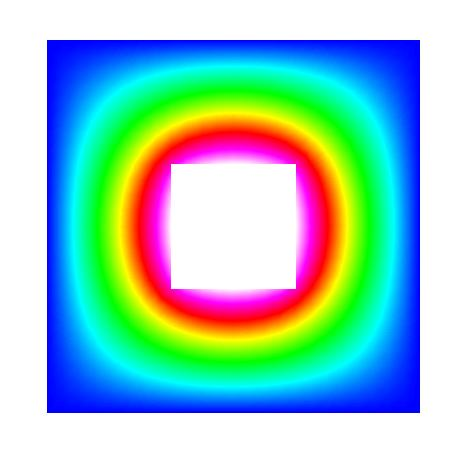
\includegraphics[width=0.4\textwidth]{temperature}
\end{center}
\caption{The temperature distribution.}
\label{f:temperature}
\end{figure}



















